%%%%%%%%%%%%%%%%%%%%%%%%%%%%%%%%%%%%%%%%%%%%%%%%%%%%%%%%%%%%%%%%%%%%%%
%
% 都市システム工学科 特別研究概要テンプレート(2015 年度版)
%
%%%%%%%%%%%%%%%%%%%%%%%%%%%%%%%%%%%%%%%%%%%%%%%%%%%%%%%%%%%%%%%%%%%%%%

\documentclass[a4paper,10pt]{jarticle}
\usepackage[dvipdfmx]{graphicx}
\usepackage{amsmath}
\usepackage{here}
\usepackage{comment}
\textwidth      18.0cm
\textheight     27.0cm
\oddsidemargin  -1.0cm
\evensidemargin -1.0cm
\topmargin      -2.3cm
\footskip        0.5cm
\columnsep       2.5zw

\renewcommand{\baselinestretch}{0.95}
\pagestyle{empty}

\makeatletter
\def\section{\@startsection {section}{1}{\z@}{-3.5ex plus -1ex minus 
 -.2ex}{2.3ex plus .2ex}{\normalsize \bf}}
\def\subsection{\@startsection {subsection}{1}{\z@}{-3.5ex plus -1ex minus 
 -.2ex}{2.3ex plus .2ex}{\normalsize \bf}}
\makeatother

\begin{document}
\twocolumn[
\begin{center}
 \vspace{-2mm}
 \begin{large}
  {\bf 流入開始時刻を考慮した地下街出入口への最適な止水板設置順序の算出}\\

 \end{large}
 \vspace{-2mm}
\end{center}
 {\bf システム最適化研究室}
 \hfill {\bf 都 13-15 馬谷 慎太郎}
 \vspace{5mm}
] %End of twocolumn

%% vspace のあとの寸法は,出来上がりイメージを見て適宜修正すること

%%%%%%%%%%%%%%%%%%%%%%%%%%%%%%%%%%%%%%%%%%%%%%%%%%%%%%%%%%%%%%%%%%%%%%
\vspace{-8mm}
\section{はじめに}
\vspace{-2.5mm}
%%%%%%%%%%%%%%%%%%%%%%%%%%%%%%%%%%%%%%%%%%%%%%%%%%%%%%%%%%%%%%%%%%%%%%

 我が国の集中豪雨の発生回数が増加傾向にあり,地下空間における浸水の危険性は高まっている.そのため地下空間の水害に着目した研究が多く行われている.

例えば,先行研究 \cite{水工学論文集2,水工学論文集1} により,事前に止水活動や避難誘導が可能であることが示されたが,具体的な止水方法については示されていない.一方武田氏の研究 \cite{武田さん卒論} では,地下空間の浸水対策として止水板の設置を考慮した上で,設置順序や設置開始するタイミングが検討された.
しかし,止水板の設置順序が最適かどうかについての検討が不十分である.

そのため本研究では,地下街の浸水対策として止水板の設置を考慮し,最適な設置順序を算出することを目的とする.ここでの最適な設置順序とは,各出入り口の流入開始時刻に間に合わなかった時間の合計が最小になるような設置順序を最適な設置順序とする.本研究では,この問題を最適化問題として定式化し,それを最適化ソルバを用いて解くことで,止水板の最適な設置順序を算出する.具体的には,梅田地下街における浸水被害の推定データを用いて数値実験を行い,止水板の最適な設置順序を算出する.
%%%%%%%%%%%%%%%%%%%%%%%%%%%%%%%%%%%%%%%%%%%%%%%%%%%%%%%%%%%%%%%%%%%%%%
\section{本研究で扱うネットワーク}
\vspace{-2mm}
 本研究で扱う最適化問題においては,止水板を設置するチームの行動を時間を追っ
て表現する必要がある.そこで本研究では,このような問題を静的に解く手段と
して広く用いられている時空間ネットワークを用いる.
時空間ネットワークとは,空間的広がりと時間的広がりを持つネットワークのことである.特に,時間方向に離散化することによって問題を静的に解く方法であり,動的に問題を解くことに比べて簡単に解を得ることができる.これを利用することにより,設置チームの動きを時間的に捉えることができる.
地下街を想定した時空間ネットワークを図 \ref{fig:zikuukann} に示す.
\vspace{-5mm}
\begin{figure}[H]
\centering
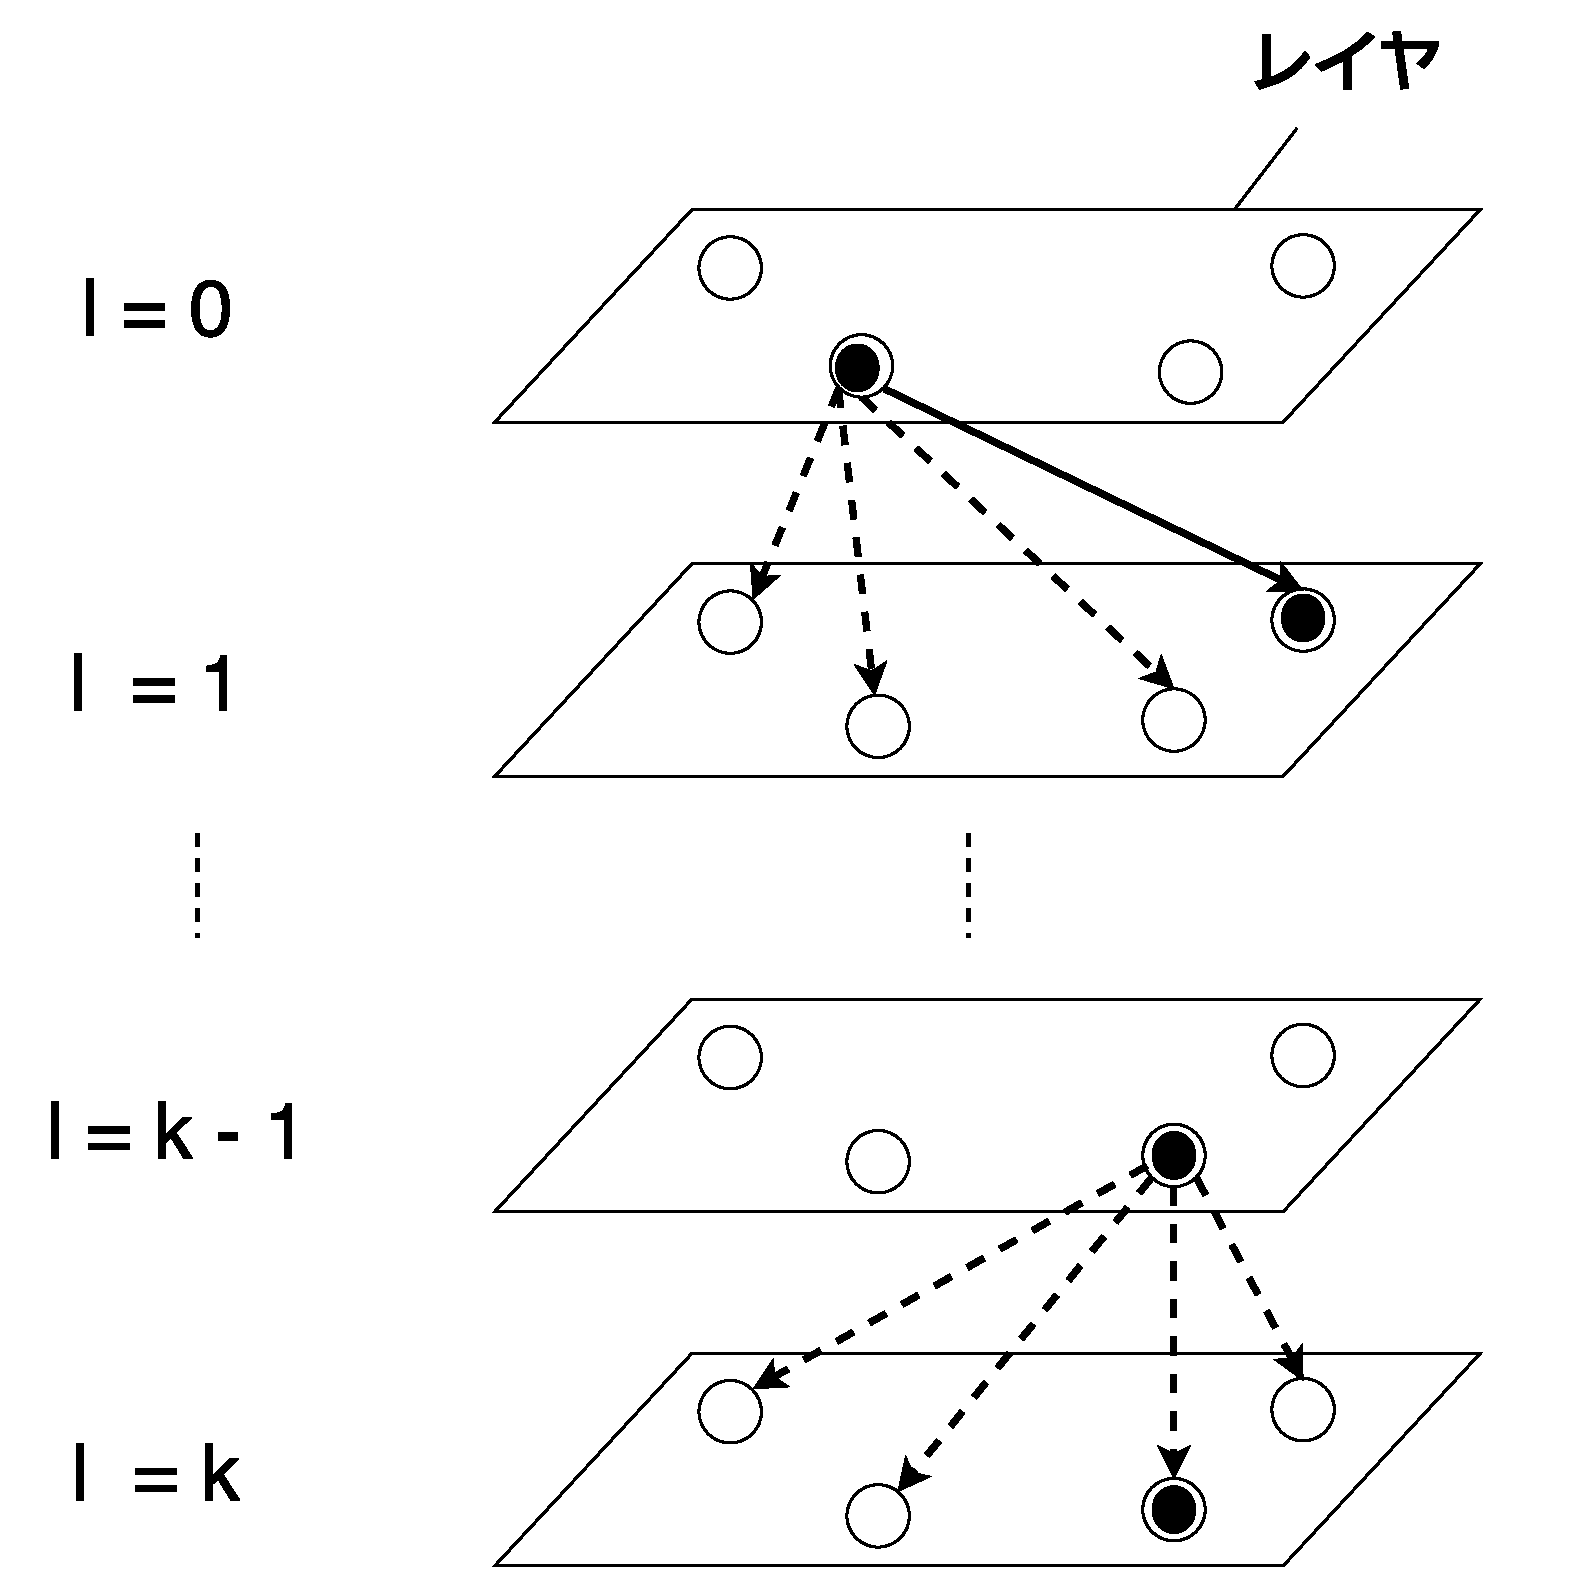
\includegraphics[scale=0.2]{./zikuukan_zu.pdf}
\caption{時空間ネットワーク図}
\vspace{-2mm}
\label{fig:zikuukann}
\end{figure}
図 \ref{fig:zikuukann} では,止水板を設置する各チームの移動回数を
$l=0,1,...k$ とし,これを時空間ネットワークにおけるレイヤに対応させる.
%
また各レイヤ上には出入口を配置し,設置チームがどの出入口に移動して止水板
を設置するかを表現できるようになっている.
%%%%%%%%%%%%%%%%%%%%%%%%%%%%%%%%%%%%%%%%%%%%%%%%%%%%%%%%%%%%%%%%%%%%%%
\vspace{-4mm}
\section{止水板最適設置問題の定式化}
\vspace{-2mm}
 本研究では,次の目的関数・制約条件をもつ止水板最適設置問題を定式化した.

本問題を定式化する際,流入時間を最小に抑えるために目的関数では,流入開始時刻に間に合わなかった出入口の止水板設置完了時刻と流入開始時刻の差の合計を最小化.\\
  \vspace{-6mm}
  \begin{description}
  \item [目的関数] 流入開始時刻に間に合わなかった出入口の止水板設置完了時刻と流入開始時刻の差の合計を最小化
    \vspace{-4mm}
  \item [制約条件1]  初期状態では,設置チームは定められたスタート地点にいる\\
    \vspace{-6mm}
  \item [制約条件2]  全出入口にはいずれかの設置チームが 1 度だけ存在する (全出入口に止水板が設置される)\\
    \vspace{-6mm}
  \item [制約条件3]  各設置チームはそれぞれの移動の際に高々 1 つの出入口に存在することができる\\
    \vspace{-6mm}
  \item [制約条件4]  枝と節点の関係性\\
    \vspace{-6mm}
  \item [制約条件5]  出入口間の移動時間を求める\\
    \vspace{-6mm}
  \item [制約条件6] 各出入口の流入開始時刻を求める\\
    \vspace{-6mm}
  \item [制約条件7]  止水板設置完了時刻と流入開始時刻の差
    \vspace{-6mm}
  \end{description}
%%%%%%%%%%%%%%%%%%%%%%%%%%%%%%%%%%%%%%%%%%%%%%%%%%%%%%%%%%%%%%%%%%%%%%

%%%%%%%%%%%%%%%%%%%%%%%%%%%%%%%%%%%%%%%%%%%%%%%%%%%%%%%%%%%%%%%%%%%%%%
\section{数値実験}
\vspace{-2mm}
\subsection{計算環境}
\vspace{-3mm}
%%%%%%%%%%%%%%%%%%%%%%%%%%%%%%%%%%%%%%%%%%%%%%%%%%%%%%%%%%%%%%%%%%%%%%

 本実験で用いた計算環境と最適化ソルバは以下の通りである:
\vspace{-4mm}
\begin{itemize}
\item OS: Microsoft Windows 10 Pro
  \vspace{-2mm}
\item CPU: Intel Core i7-6950X CPU @ 3.00GHz 3.00GHz
  \vspace{-7mm}
\item メモリ:64.00GB
   \vspace{-2mm}
 \item ソルバ:Gurobi Optimizer
\end{itemize}
\vspace{-8mm}
%\begin{figure}[htpb]
% \begin{center}
%  
\includegraphics[scale=0.3]{./KU.eps}
%  \caption{図や写真等のタイトルは下に配置}
%  \label{fig:1}
% \end{center}
%\end{figure}
%%%%%%%%%%%%%%%%%%%%%%%%%%%%%%%%%%%%%%%%%%%%%%%%%%%%%%%%%%%%%%%%%%%%%%
\subsection{実験 1:基本ケース}
\vspace{-2mm}
%%%%%%%%%%%%%%%%%%%%%%%%%%%%%%%%%%%%%%%%%%%%%%%%%%%%%%%%%%%%%%%%%%%%%%

 実験 1 では,以下の条件で計算を行った:
\vspace{-3mm}
\begin{table}[H]
 \begin{center}
   \caption{実験 1 で設定した条件}
  \begin{tabular}{ll}
   \hline
   1 時間あたりの降雨量 & 60mm \\
   排水用ポンプ & 機能停止 \\
   雨水が流入する出入口の数 & 24 箇所 \\
   止水板設置チーム数 & 6 チーム \\
   止水板設置チームの歩行速度 & 66 m/分  \\
   降雨開始から止水板設置開始までの時間 & 60 分 \\
   止水板 1 箇所の設置に要する時間 & 3 分 \\
   \hline
  \end{tabular}
  \label{tb:ex1}
 \end{center}
\end{table}
\vspace{-6mm}
止水板設置の対象となる出入口を図 \ref{fig:umedamap} に示す.これは,関西大学・岡部史弥氏の計算によるもので,
1 時間あたりの降雨量が 60 mmの時,排水用ポンプが稼働してなかったときに雨水が流入すると推定される地下街出入口である.
本実験では,これらに対し,6 チームで止水板の設置することを想定する.止水板の設置は降雨開始直後に設置し始めるものではないため,
本実験では降雨開始から止水板設置開始までの時間を 60 分と想定する.なお,大阪地下街防災センターの近くにある出入口をスタート地点としている.
\begin{figure}[H]
  \begin{tabular}{cc}
  \begin{minipage}{0.5\hsize}
  \begin{center}
    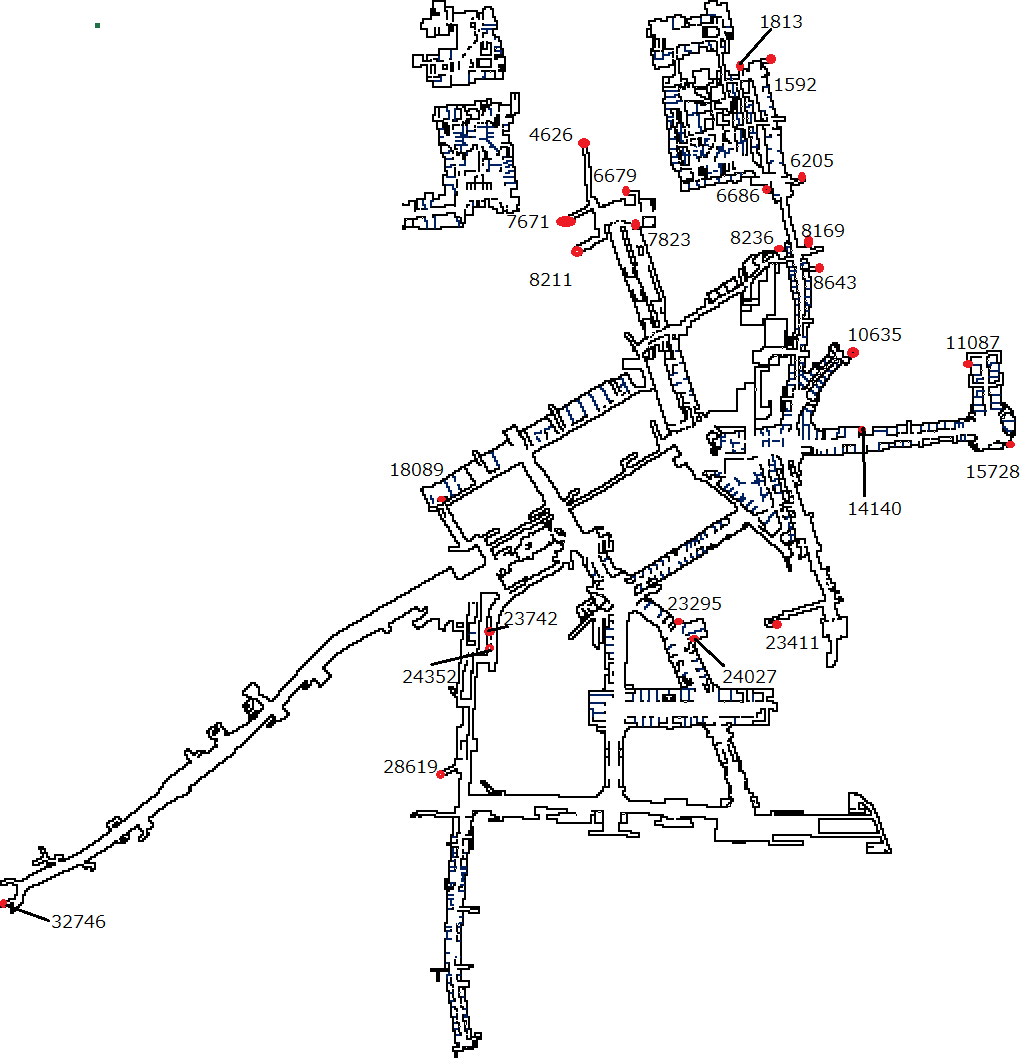
\includegraphics[width=30mm]{umedamap.png}
  \end{center}
  \vspace{-5.2mm}
\caption{出入口流入箇所}
\label{fig:zikken2_4team_gurahu}
\end{minipage}
\begin{minipage}{0.5\hsize}
\begin{center}
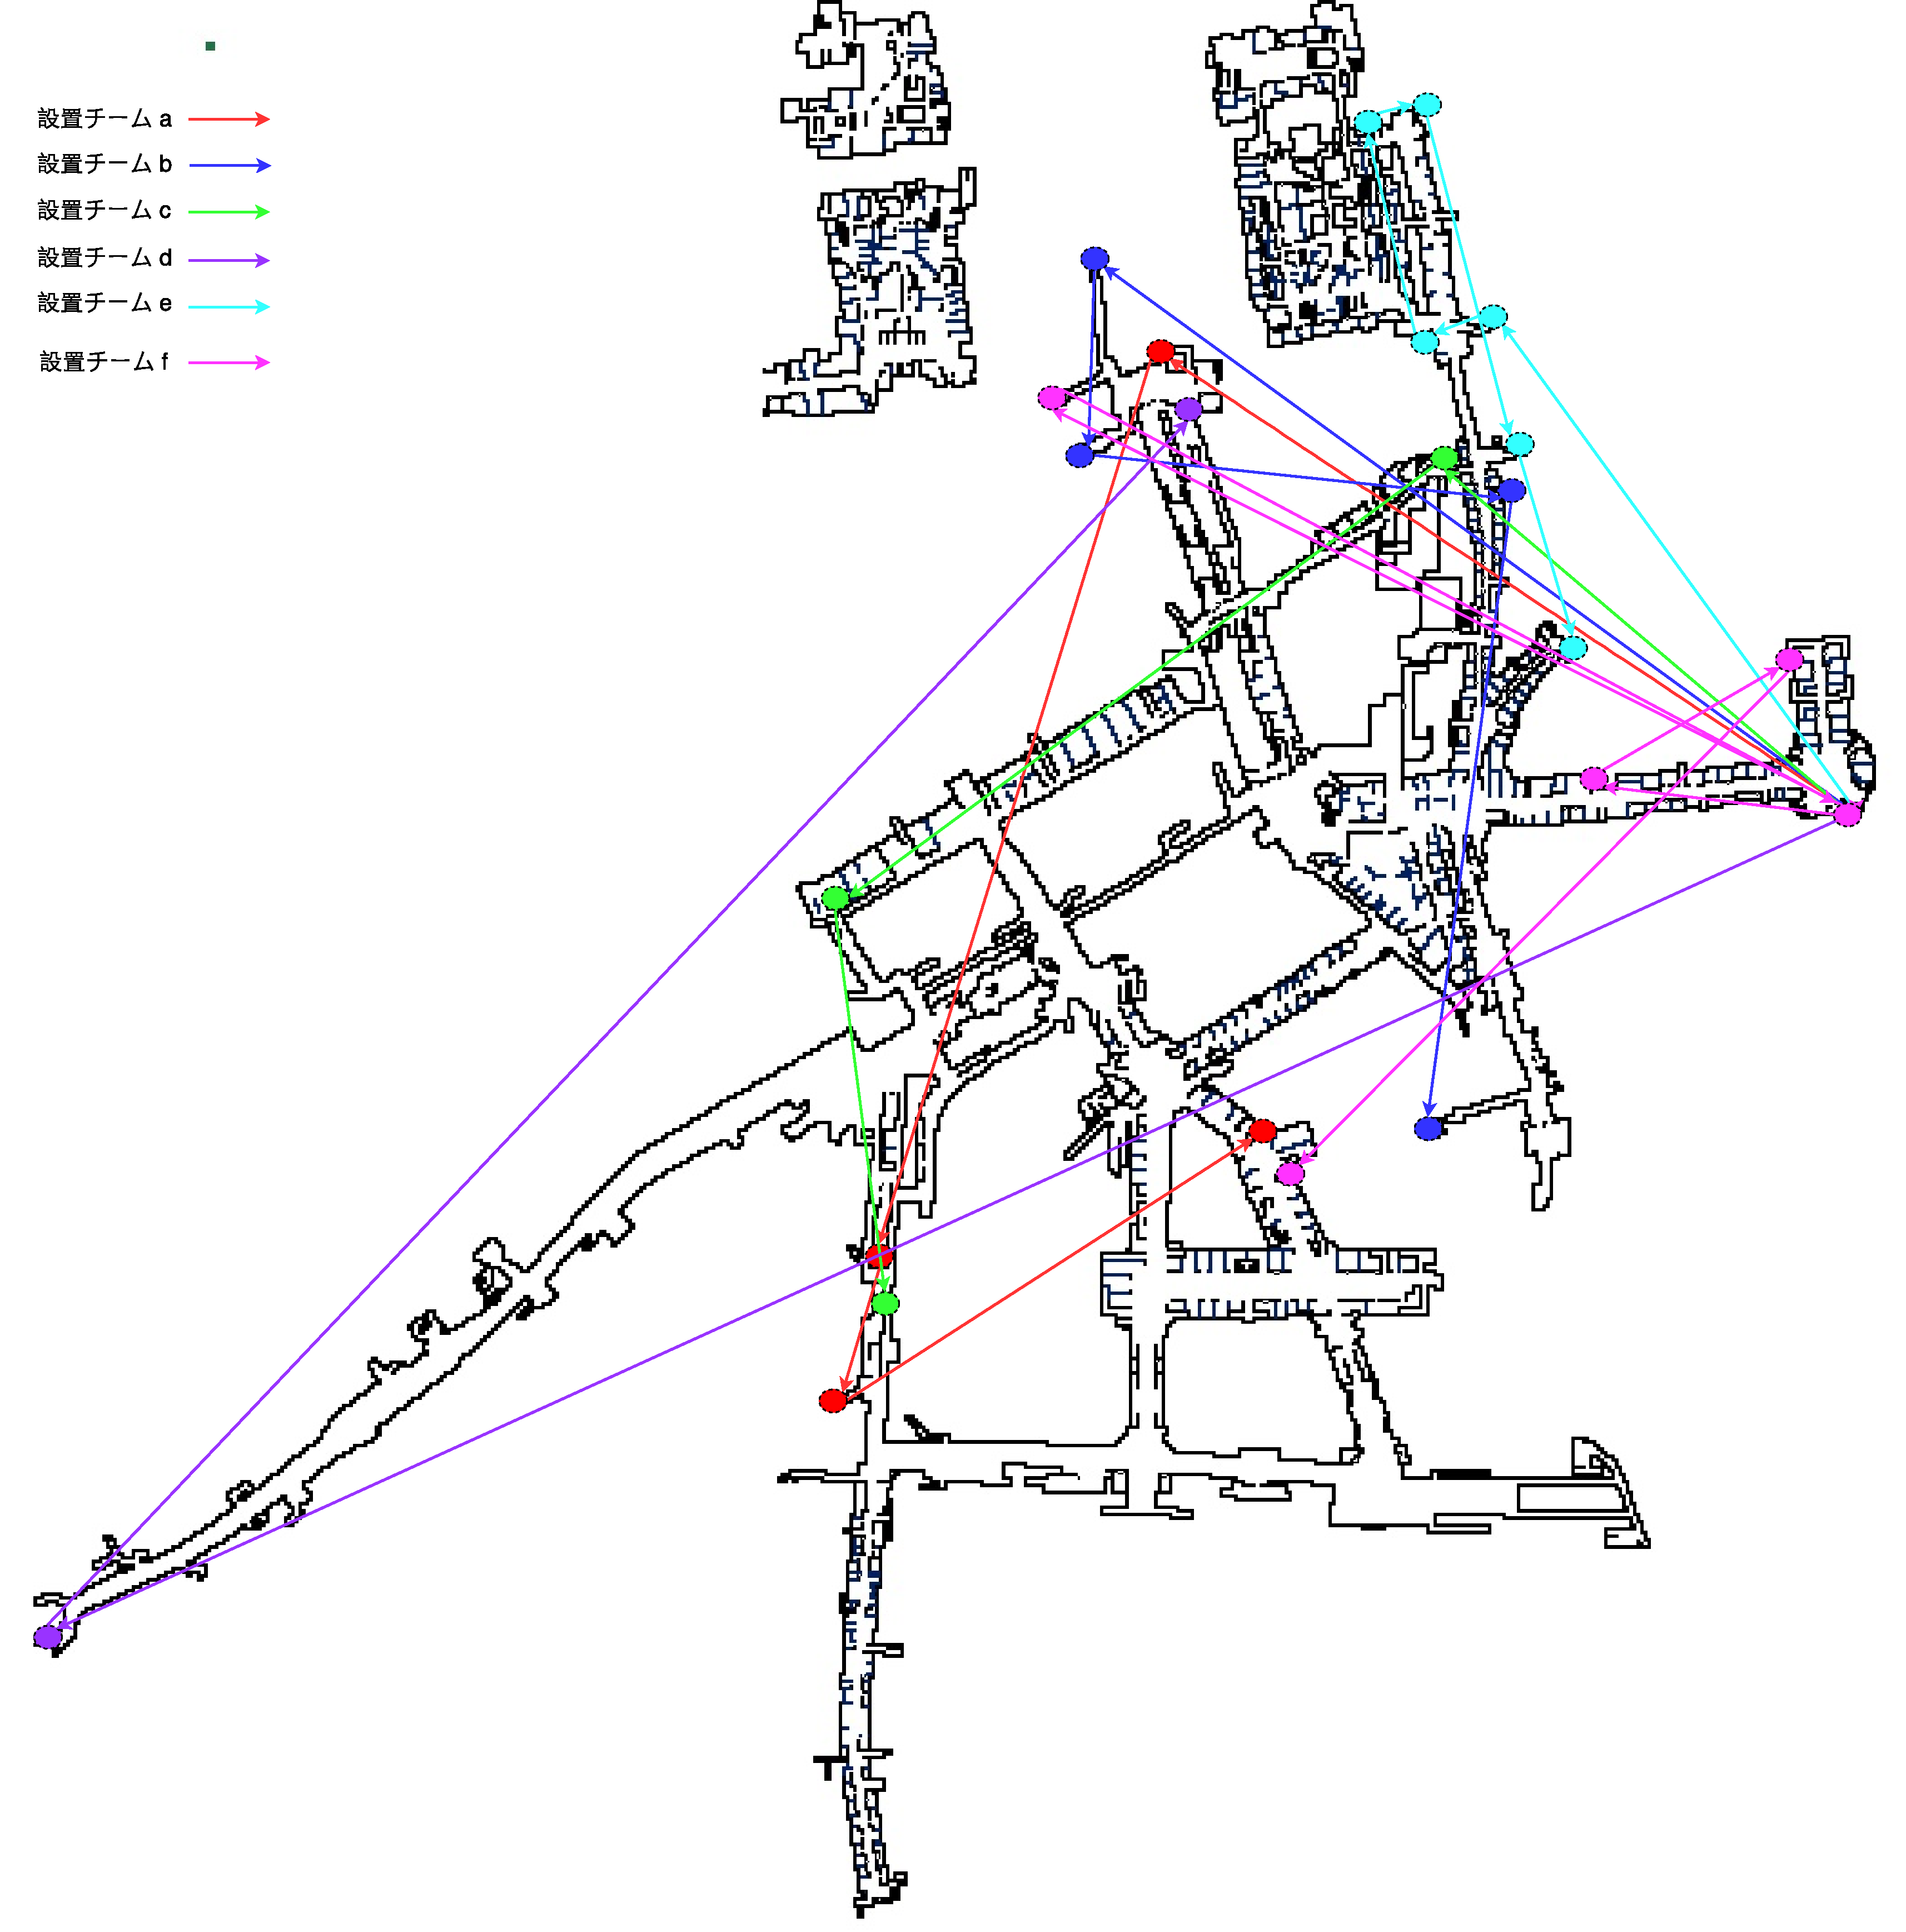
\includegraphics[width=30mm]{zikken1_settizyunzyo_map.pdf}
\end{center}
\vspace{-5.2mm}
\caption{最適設置順序 (実験 1)}
\label{fig:zikken2_5team_gurahu}
\end{minipage}
\end{tabular}
\end{figure}
\vspace{-4mm}
\begin{figure}[H]
\centering
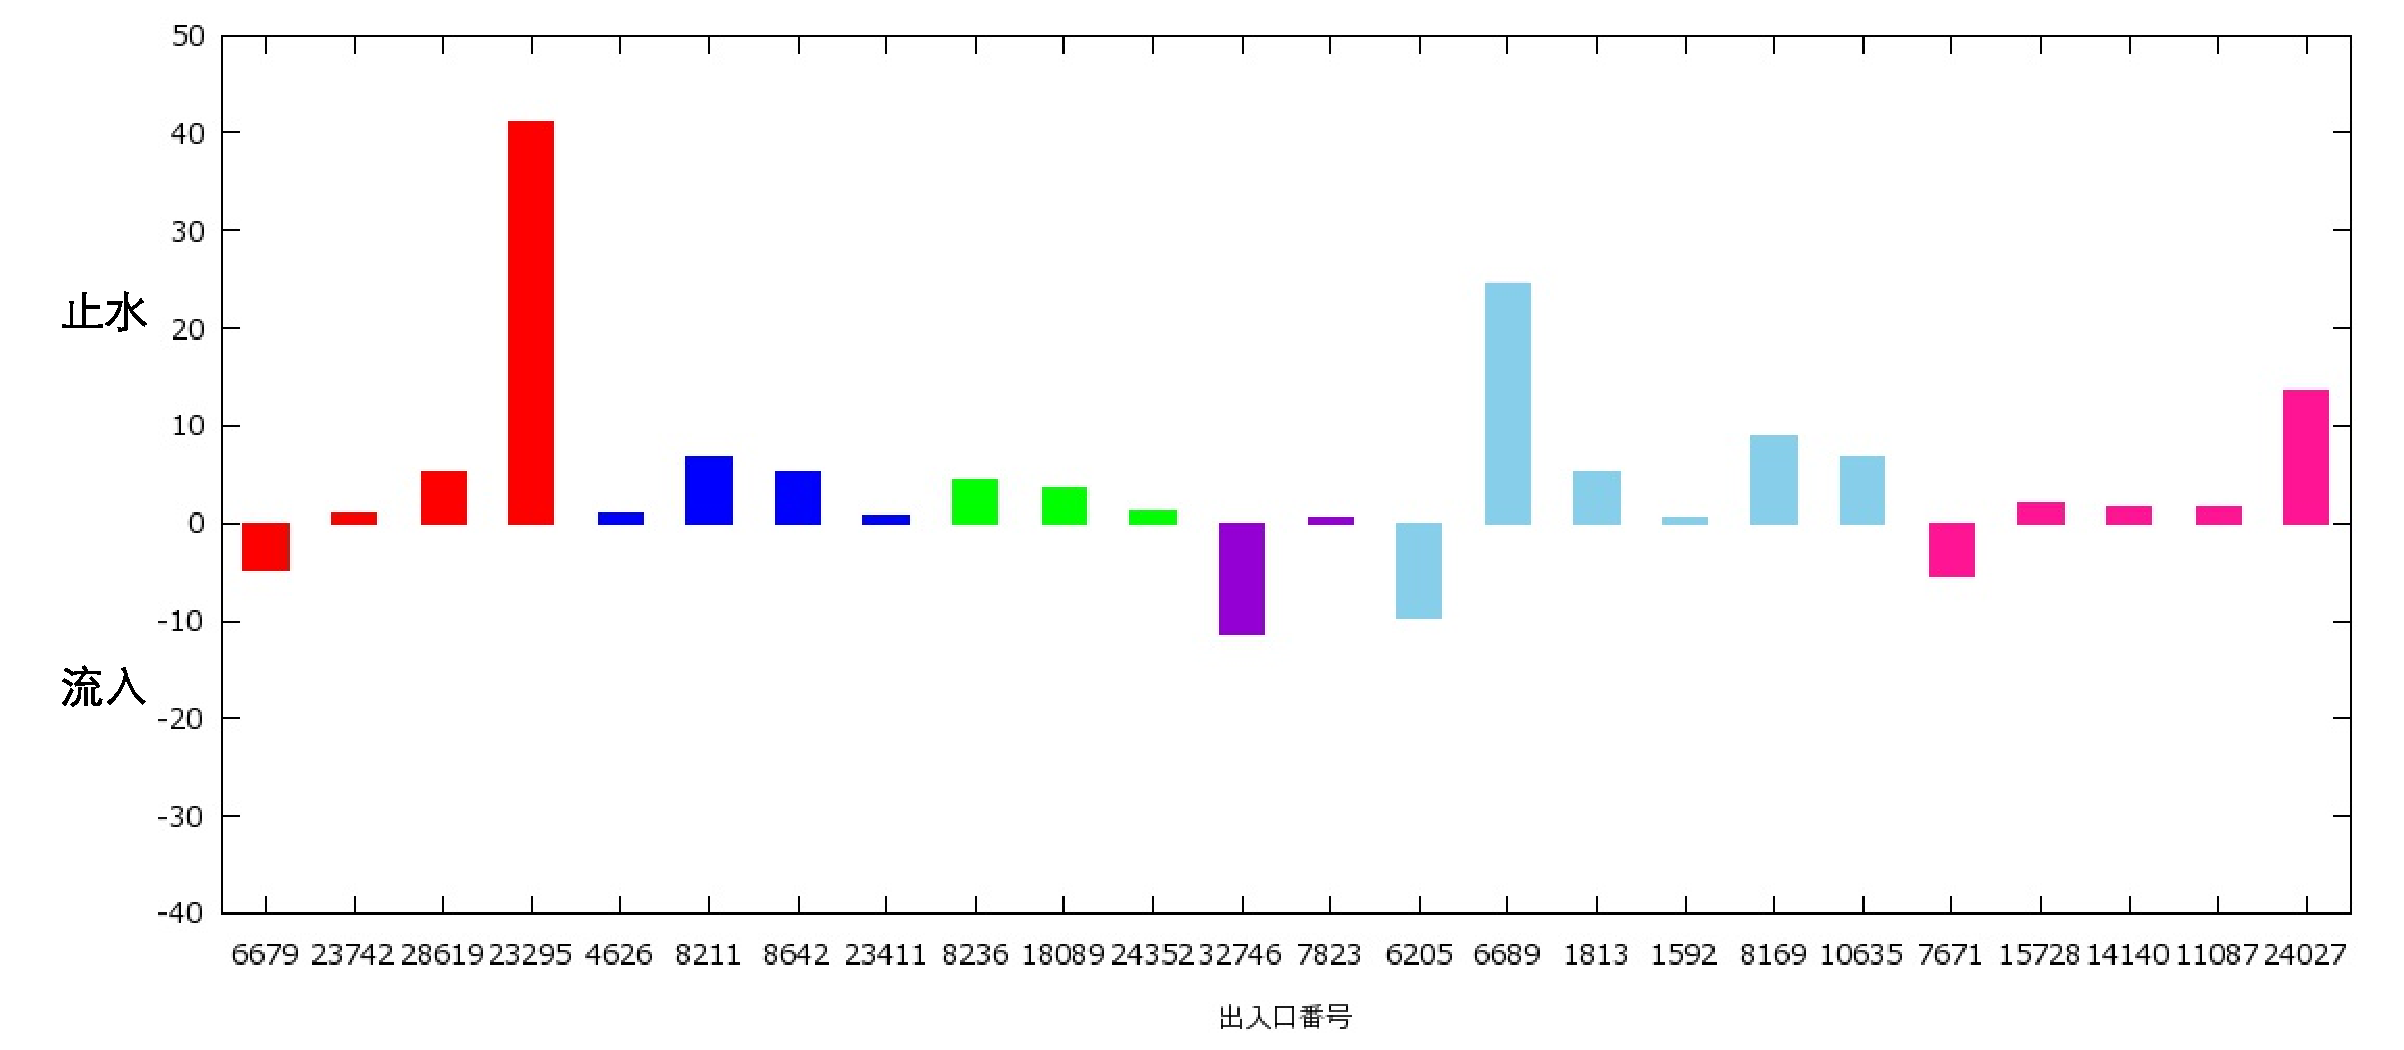
\includegraphics[scale=0.2]{zikken1_gurahu}
\vspace{-4mm}
\caption{梅田地下街 流入状況 }
\label{fig:zikken1_gurahu}
\end{figure}
図 \ref{fig:zikken1_gurahu} (また,5 ,6 ,7) は止水板を設置すべき各出入口に対して,「(流入開始時刻)$-$(止水板設置完了時刻)」をグラフ化したものである.
すなわち,グラフが零より上にある場合,その出入口への設置は流入開始時刻に間に合っており,零より下であればその分だけ流入していることを表している.
また,同一色のグラフは,同一のチームが止水板を設置していることを表し,一つのチーム内では設置を行った出入口順に左から並べている.

実験 1 の図 \ref{fig:zikken2_5team_gurahu} を見ると,比較的近い出入り口を設置する設置チームや長い距離を移動しているため,少数の出入口のみ設置している設置ームがあることが分かる.
\vspace{-4mm}
%%%%%%%%%%%%%%%%%%%%%%%%%%%%%%%%%%%%%%%%%%%%%%%%%%%%%%%
\subsection{実験 2 : 止水板設置チームの数を変更}
\vspace{-2mm}
%%%%%%%%%%%%%%%%%%%%%%%%%%%%%%%%%%%%%%%%%%%%%%%%%%%%%%%%%%%%%%%%%%%%%%
 実験 2 では,実験 1 の設定 (表 \ref{tb:ex1}) のうち,止水板設置チームの数を 4組, 5組, 7組 に変えて実験を行い,チーム数を
変えた時の変化を検証した.
\vspace{-4mm}
\begin{figure}[H]
\centering
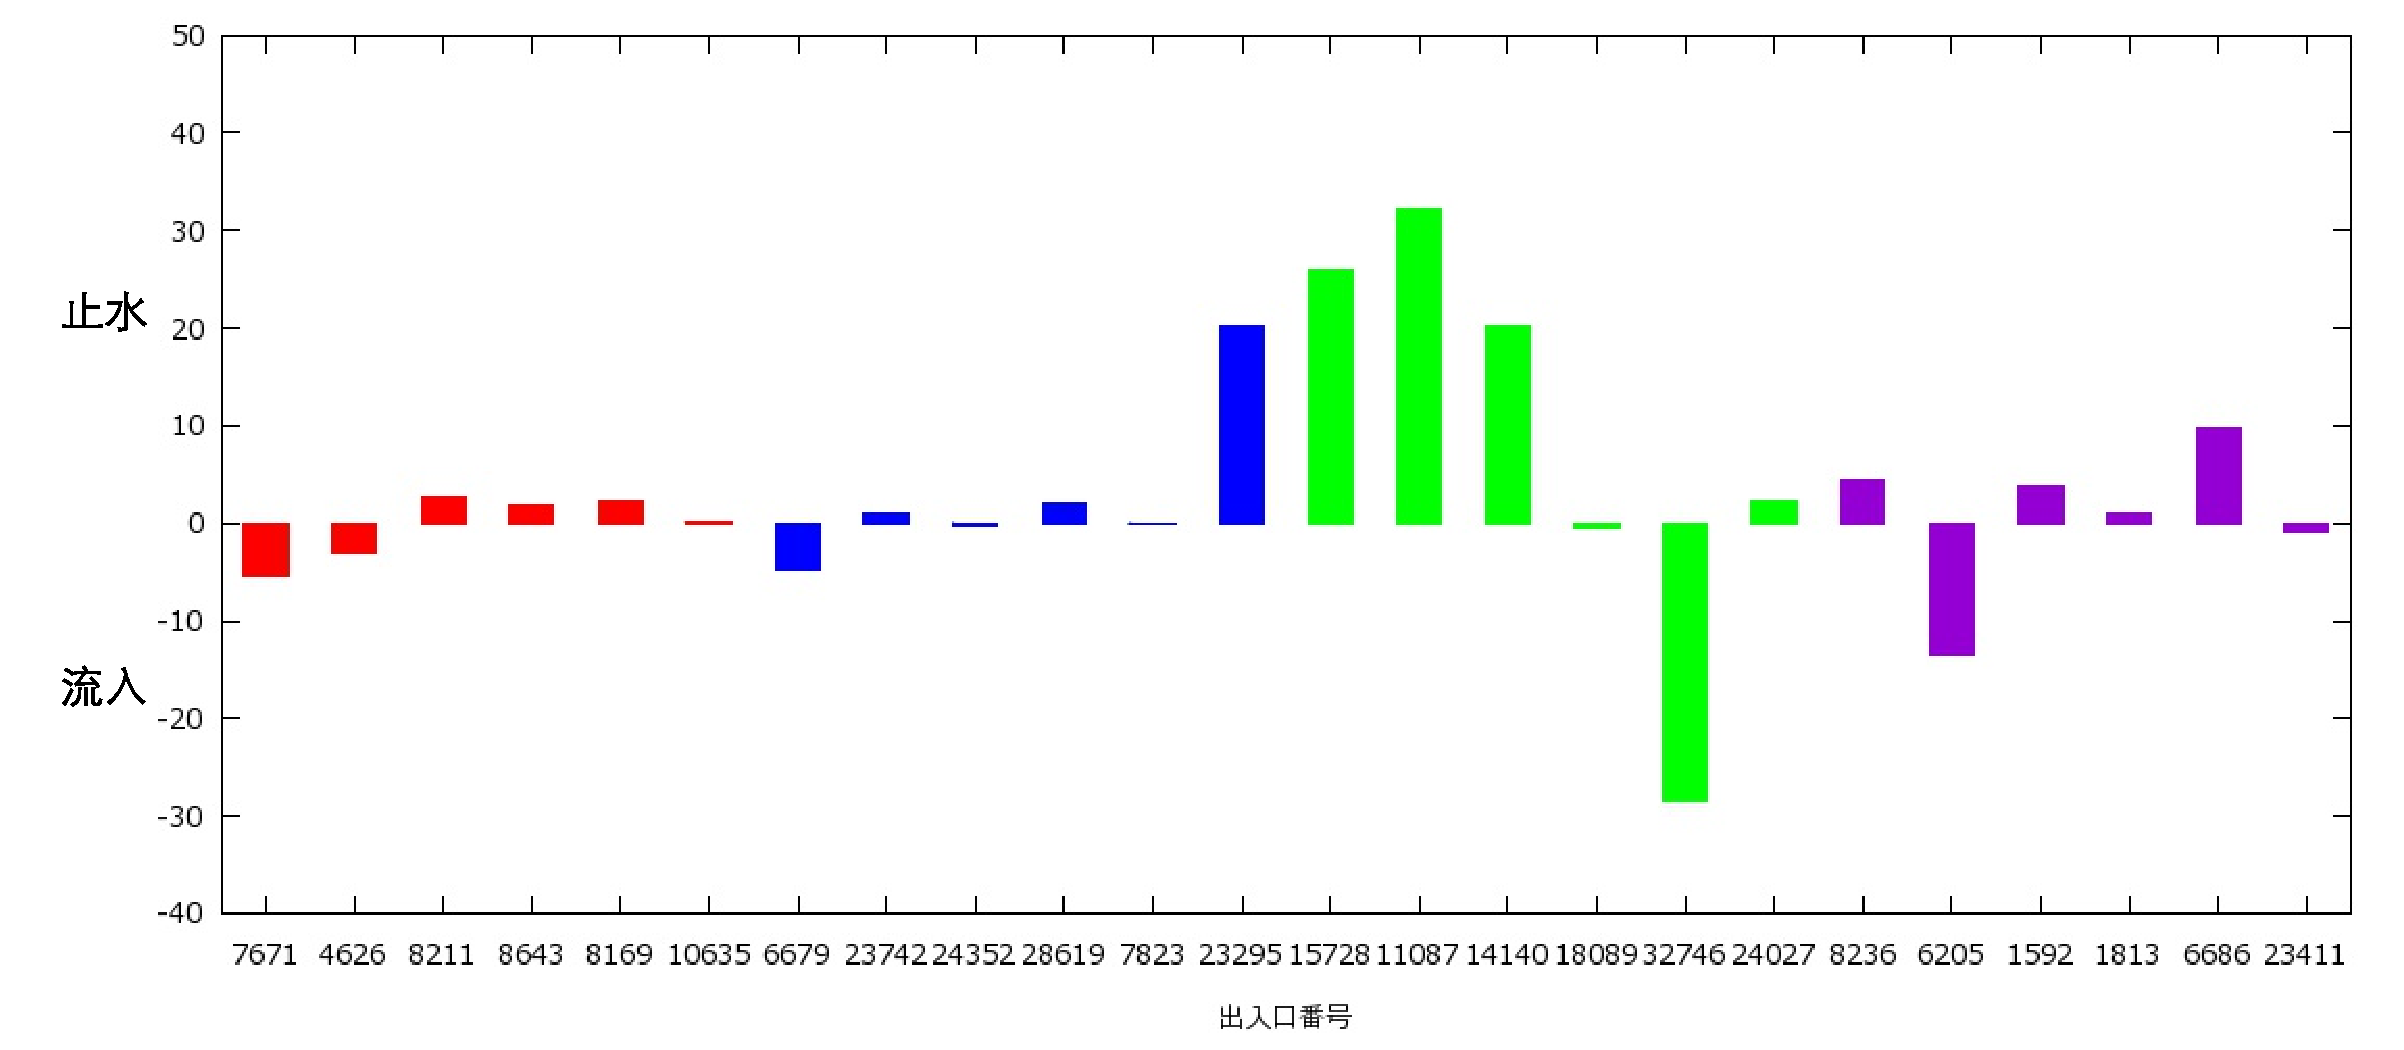
\includegraphics[scale=0.2]{zikken2_4team_gurahu.pdf}
\vspace{-4mm}
\caption{設置チーム4組の流入状況}
\label{fig:zikken2_4team_gurahu}
\end{figure}
\vspace{-4mm}
\begin{figure}[H]
\centering
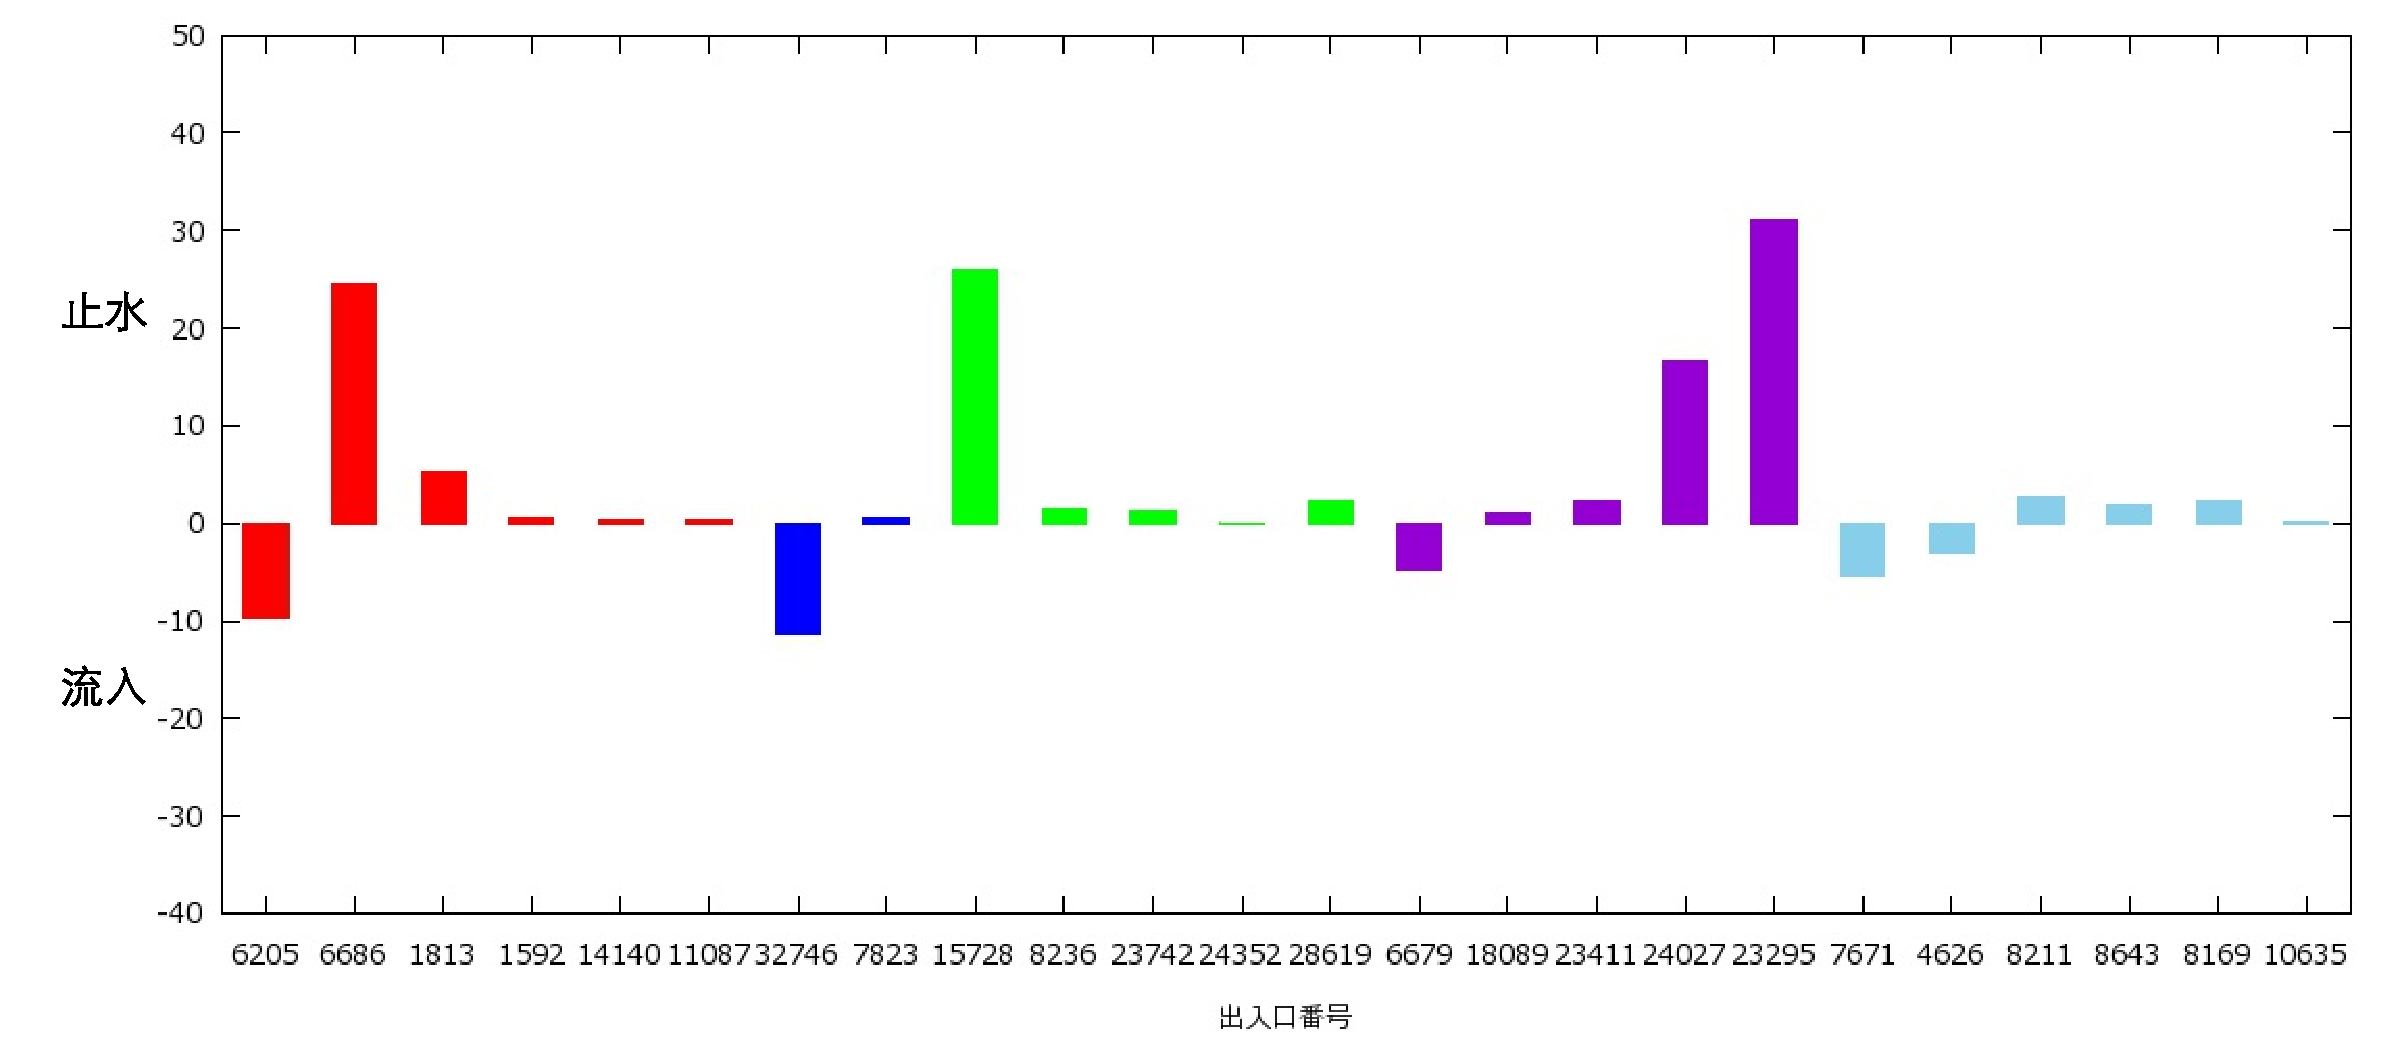
\includegraphics[scale=0.2]{zikken2_5team_gurahu.pdf}
\vspace{-4mm}
\caption{設置チーム5組の流入状況}
\label{fig:zikken2_5team_gurahu}
\end{figure}
\vspace{-4mm}
\begin{figure}[H]
\centering
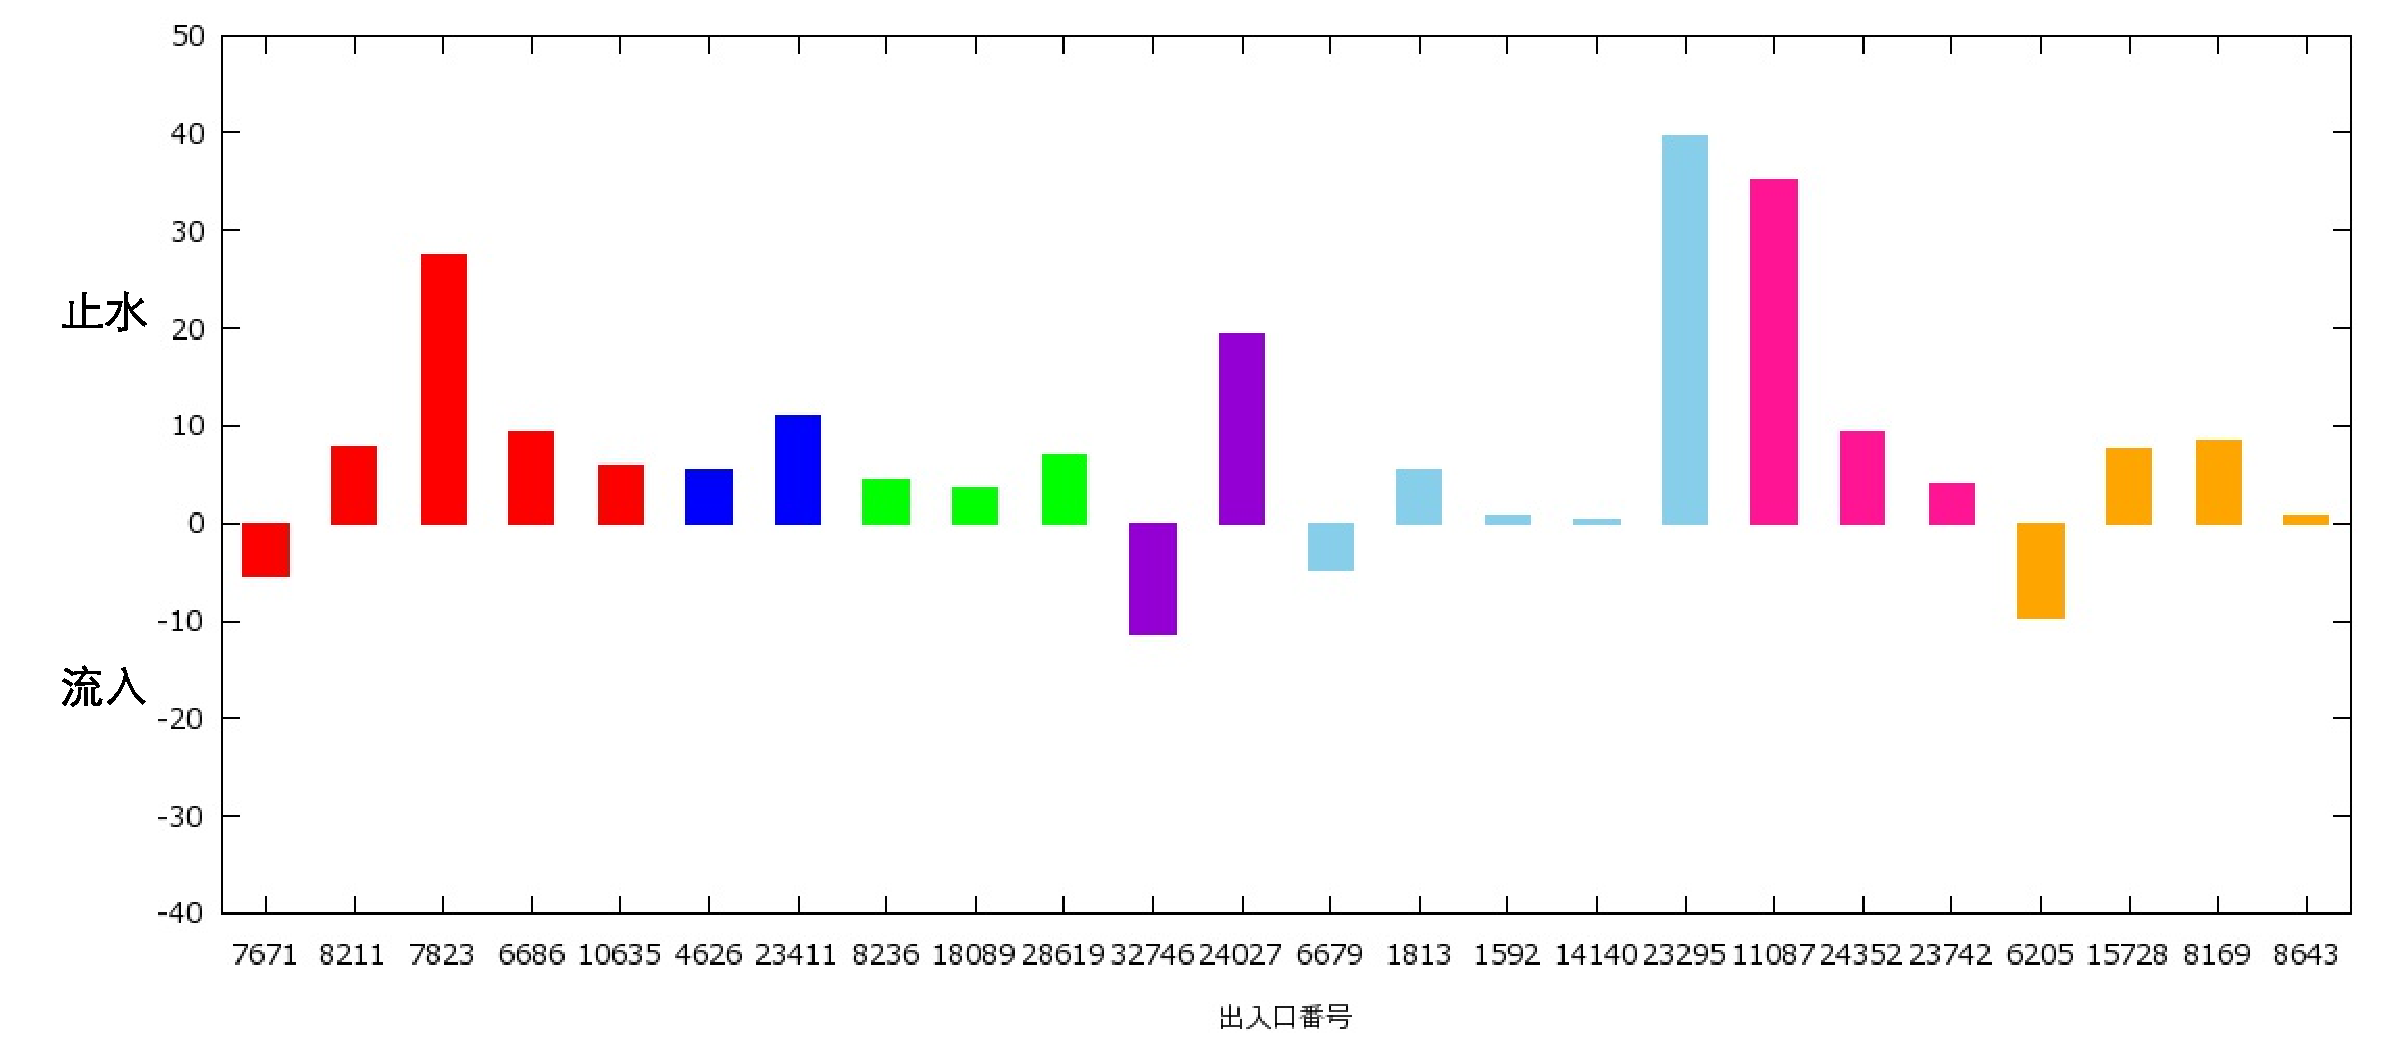
\includegraphics[scale=0.2]{zikken2_7team_gurahu.pdf}
\vspace{-4mm}
\caption{設置チーム7組の流入状況}
\label{fig:zikken2_7team_gurahu}
\end{figure}
 実験 2 では次のことが分かった.
\begin{itemize}
\item 図 \ref{fig:zikken2_4team_gurahu} \ref{fig:zikken2_5team_gurahu} \ref{fig:zikken2_7team_gurahu} より,設置チームの数が多いと各出入口の流入開始時刻までに余裕をもって設置している出入口が多い.逆に,設置チームの数が少ないと流入開始時刻ぎりぎりのところで設置している出入口が多い.
  \vspace{-2mm}
\item 止水板設置チームの数が増えるほど地下街に流入する時間は短くなるが,ある一定の数まで増えると地下街に流入する時間は変化がなくなる.
\end{itemize}
\begin{comment}
\begin{table}[H]
\begin{center}
\caption{実験 2 結果 まとめ}
 \begin{tabular}{lrrrrr}\hline
      チーム数   & 計算時間(s) & GAP(\%) & 目的関数\\\hline
         4     &  86402 & 9.14 & 57.06\\
         5     &  59610 & 0.02 & 34.55\\
         6     &  20875 & 0.03 & 31.36\\
         7     &  1446  & 4.73 & 31.36\\\hline
\end{tabular}
    \label{tb:実験2_team}
\end{center}
\end{table}
 \end{comment}
\begin{figure}[H]
\centering
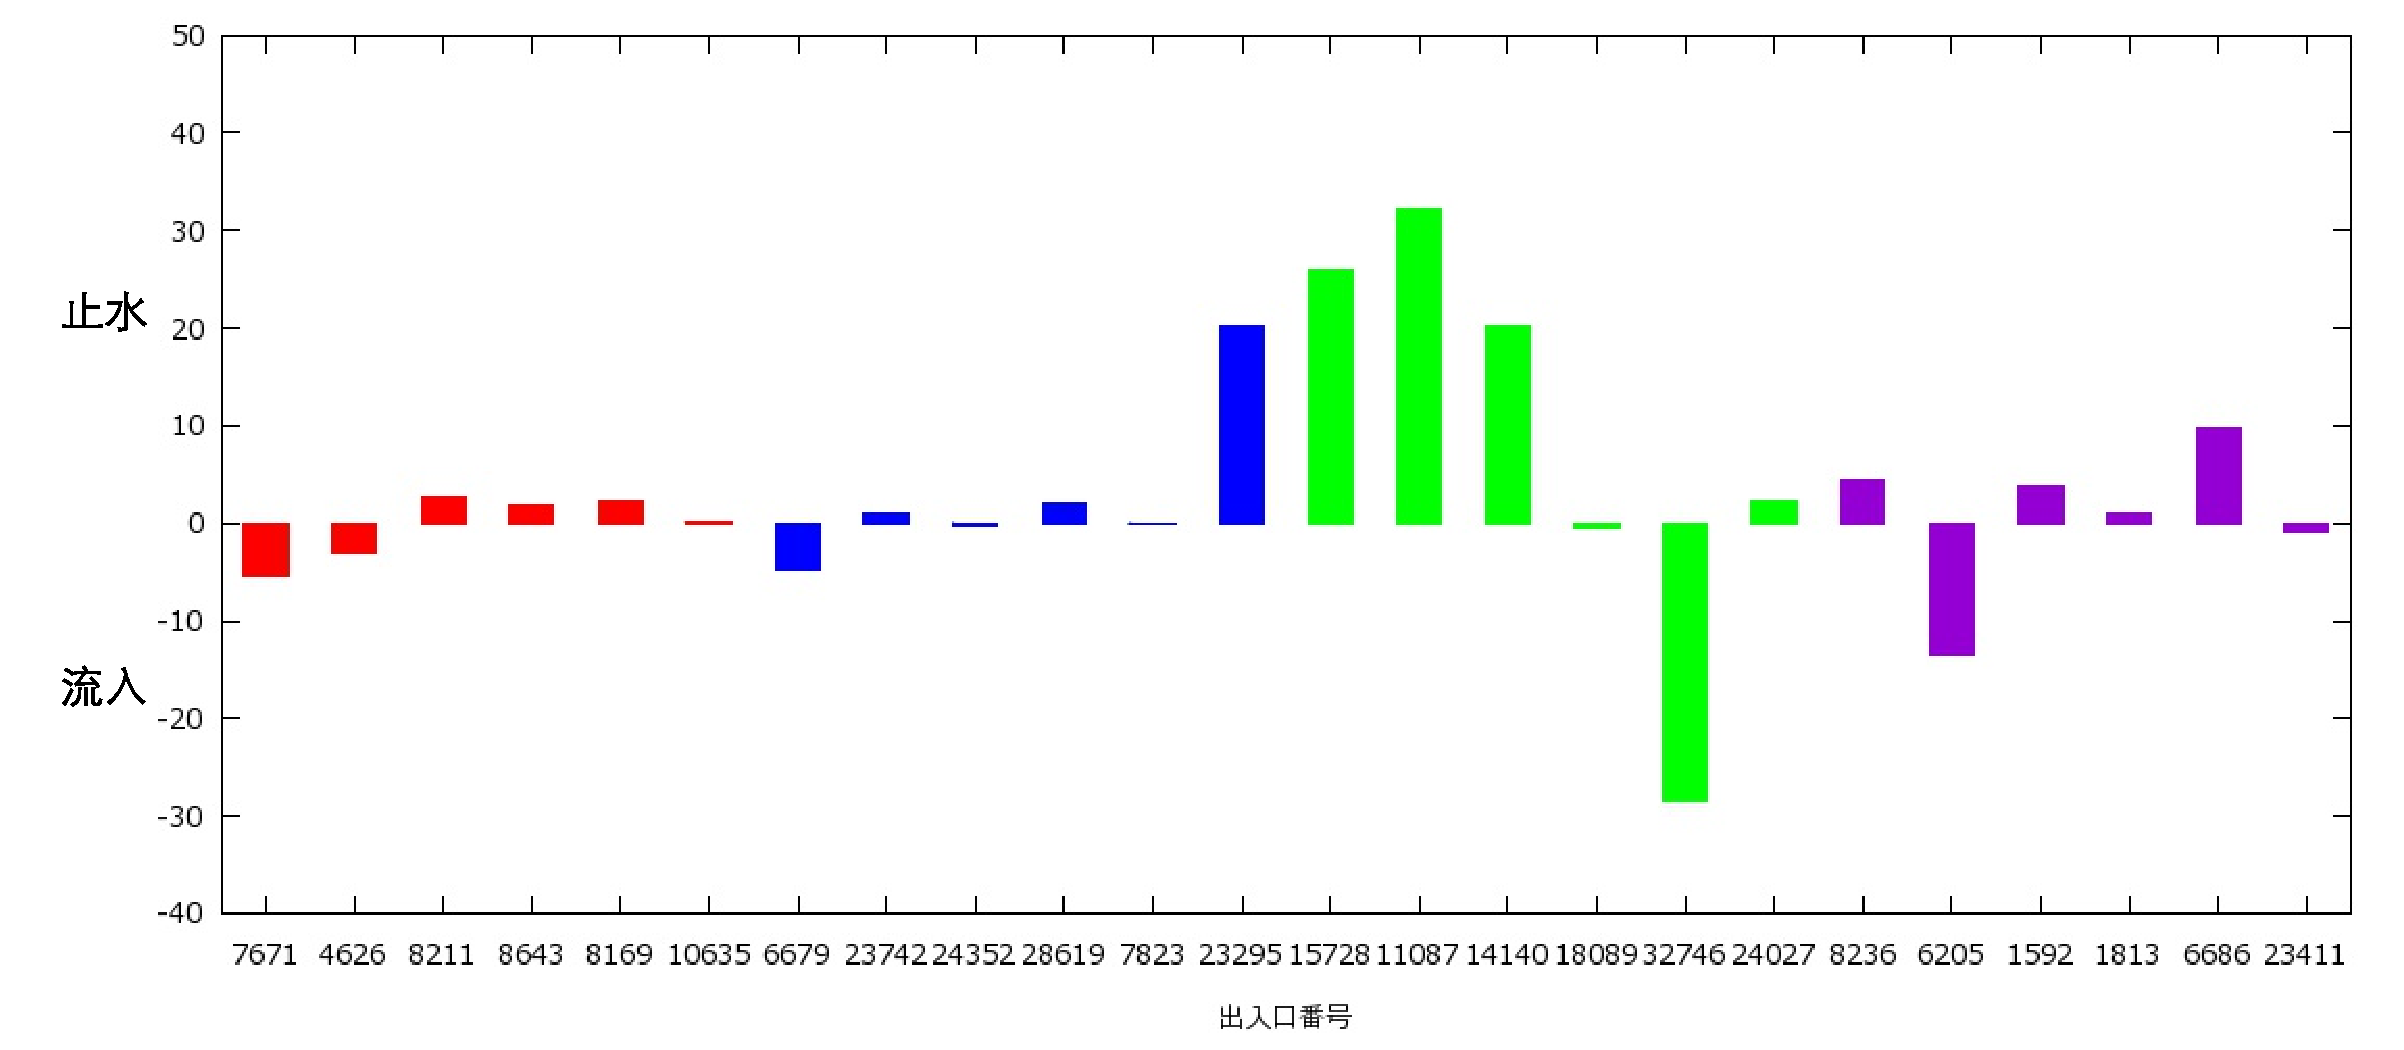
\includegraphics[scale=0.25]{zikken2_4team_gurahu.pdf}
\caption{梅田地下街 流入状況 }
\vspace{-2mm}
\label{fig:zikken2_4team_gurahu.pdf}
\end{figure}
\vspace{-5mm}
 表 \ref{tb:実験2_team} より,止水板設置チームの数が増える度に流入開始時刻に間に合わなかった時間の合計が
    短くなっていることが分かる.ただし,設置チーム 6 から 7 に増やしても流入開始時刻に間に合わなかった時間の合計に
    変化はないことが分かった.このことから設置チームが増えるたびに流入開始時刻に間に合わなかった時間の合計は
    短くなるが,その効果には上限があることが推定される.
    \vspace{-5mm}
%%%%%%%%%%%%%%%%%%%%%%%%%%%%%%%%%%%%%%%%%%%%%%%%%%%%%%%%%%%%%%%%%%%%%%
\vspace{-4mm}
\subsection{実験 3}
\vspace{-10mm}
%%%%%%%%%%%%%%%%%%%%%%%%%%%%%%%%%%%%%%%%%%%%%%%%%%%%%%%%%%%%%%%%%%%%%%

\begin{table}[H]
\begin{center}
\caption{実験 3 結果 まとめ}
 \begin{tabular}{lrrrrr}\hline
   設置開始& 計算時間(s) & GAP(\%) & 目的関数\\\hline
         50     &  306   & 29.2 & 1.45\\
         60     &  20875 & 0.03 & 31.36\\
         70     &  86400 & 22.9 & 110.48\\\hline
    \end{tabular}
    \label{tb:実験3_settikaisi}
\end{center}
\end{table}
\vspace{-5mm}
表 \ref{tb:実験3_settikaisi} より,降雨開始から止水板を設置し始めるまでの時間が長いほど地下街に流入する時間が増える.また,降雨開始
から止水板を設置するまでの時間が遅くなると地下街に流入する時間が大幅に増える.
%%%%%%%%%%%%%%%%%%%%%%%%%%%%%%%%%%%%%%%%%%%%%%%%%%%%%%%%%%%%%%%%%%%%%%
\subsection{実験 4}
\vspace{-10mm}
%%%%%%%%%%%%%%%%%%%%%%%%%%%%%%%%%%%%%%%%%%%%%%%%%%%%%%%%%%%%%%%%%%%%%%

\begin{table}[H]
\begin{center}
\caption{実験 4 結果 まとめ}
 \begin{tabular}{lrrrrr}\hline
      移動速度(m/s)  &計算時間(s) & GAP(\%) & 目的関数\\\hline
         50      &  86400 & 17.5 & 60.60\\
         60      &  86400 & 6.73 & 39.13\\
         66      &  20875 & 0.03 & 31.36\\
         72      &  615   & 4.53 & 27.17\\\hline
    \end{tabular}
    \label{tb:実験4_idousokudo}
\end{center}
\end{table}
\vspace{-5mm}
 表 \ref{tb:実験4_idousokudo} より,移動速度が大きくなるほど
地下街に流入する時間は短くなる.ただし,移動速度が向上するほど雨水流入時間の現象に及ぼす効果が小
さくなっていることがわかる.
%%%%%%%%%%%%%%%%%%%%%%%%%%%%%%%%%%%%%%%%%%%%%%%%%%%%%%%%%%%%%%%%%%%%%%
\vspace{-5mm}
\begin{comment}
\subsection{実験 5}
\vspace{-10mm}
%%%%%%%%%%%%%%%%%%%%%%%%%%%%%%%%%%%%%%%%%%%%%%%%%%%%%%%%%%%%%%%%%%%%%%
\begin{table}[H]
\begin{center}
\caption{実験 5 結果 まとめ}
 \begin{tabular}{lrrrrr}\hline
      設置時間(分) & 計算時間(s)& GAP(\%) & $d_{l,p}$\\\hline
           3   &  20875 & 0.03 & 31.36\\
           5   &  36863 & 0.00  & 47.45\\\hline
    \end{tabular}
    \label{tb:実験5_settizikan}
\end{center}
\end{table}
\vspace{-10mm}
 表 \ref{tb:実験5_settizikan} より,止水板設置に要する時間が増えると地下街に流入する時間も増える.
%%%%%%%%%%%%%%%%%%%%%%%%%%%%%%%%%%%%%%%%%%%%%%%%%%%%%%%%%%%%%%%%%%%%%%
\vspace{-10mm}
\end{comment}
\section{おわりに}
%%%%%%%%%%%%%%%%%%%%%%%%%%%%%%%%%%%%%%%%%%%%%%%%%%%%%%%%%%%%%%%%%%%%%

%%%%%%%%%%%%%%%%%%%%%%%%%%%%%%%%%%%%%%%%%%%%%%%%%%%%%%%%%%%%%%%%%%%%%
% 数式は,\verb|align| 環境を用いて入力すること.
%
%\begin{align}
% G &= \sum_{n = 0}^\infty b_n(t)
% \label{eq:G} \\
% F &= \int_\Gamma \sin z \; {\rm d}z
% \label{eq:F}
%\end{align}
%
%%%%%%%%%%%%%%%%%%%%%%%%%%%%%% 
%%%%%%%%%%%%%%%%%%%%%%%%%%%%%%
\begin{comment}

\begin{table}
 \begin{center}
  \caption{表のタイトルは上に配置}
  \begin{tabular}{|l|l|l|}
   \hline
   A \hspace{2cm} & B \hspace{2cm} & C \hspace{2cm} \\
   \hline
   あ & い & う \\
   \hline
  \end{tabular}
  \label{tb:1}
 \end{center}
\end{table}

\end{comment}
%%%%%%%%%%%%%%%%%%%%%%%%%%%%%%%%%%%%%%%%%%%%%%%%%%%%%%%%%%%%%%%%%%%%%%
%%%%%%%%%%%%%%%%%%%%%%%%%%%%%%%%%%%%%%%%%%%%%%%%%%%%%%%%%%%%%%%%%%%%%%
\begin{comment}
文献や式・図表の引用は以下のように:
\begin{itemize}
 \item \cite{都市12}
 \item 式 (\ref{eq:G})
 \item 図 \ref{fig:1}
 \item 表 \ref{tb:1}
\end{itemize}
\end{comment}
%%%%%%%%%%%%%%%%%%%%%%%%%%%%%%%%%%%%%%%%%%%%%%%%%%%%%%%%%%%%%%%%%%%%%
\begin{thebibliography}{9}
\vspace{-2.5mm}
\bibitem{水工学論文集2}井上知美,川中龍児,石垣泰輔,尾崎平,戸田圭一,内水氾濫による大規模地下街の浸水過程と避難の安全性に関する検討,水工学論文集 , $55$, s$973$-s$978$ ($2011$).
\vspace{-2mm}
\bibitem{水工学論文集1}森兼政行,石垣泰輔,尾崎平,戸田圭一,大規模地下空間を有する都市域における地下空間への内水氾濫水の流入特性とその対策,水工学論文集 , $55$, s967-s972 ($2011$).
  \vspace{-2mm}
\bibitem{武田さん卒論}武田侑也,大規模地下空間における内水氾濫による浸水対策の検討,関西大学環境都市工学部 $2015$ 年度卒業論文 ($2016$).  
\end{thebibliography}
%%%%%%%%%%%%%%%%%%%%%%%%%%%%%%%%%%%%%%%%%%%%%%%%%%%%%%%%%%%%%%%%%%%%%%

\end{document}

%%%%% End of file %%%%%

